\newpage

\chapter{Requirements and Analysis}
In response to the pressing need for seamless healthcare monitoring, this project introduces VitalMonitor, a centralized system designed to enhance real-time monitoring of healthcare professional (HCP) vitals. This innovative IoTaaS platform comprises two key components: the Smart Patch, a wearable IoT device for vital sensing, and a comprehensive dashboard for monitoring and managing healthcare professionals. VitalMonitor not only simplifies access to vital health metrics but also integrates these functionalities into a user-friendly platform, minimizing the technological burden on healthcare organizations and easily integrate into their exisiting workflow. The chapter covers on the required features of the system and an evaluation system for the system is introduced.

\section{VitalMonitor}

VitalMonitor marks a significant advancement in healthcare technology by prioritizing the well-being of HCPs in high-stress environments. This system includes the Smart Patch, a discrete, non-intrusive wearable device tailored for healthcare settings, and a web-based dashboard that facilitates real-time data analysis and monitoring. The goal is to deliver actionable insights into HCP health, enabling timely interventions to alleviate stress and fatigue, and thereby enhancing patient care and safety.


Passive monitoring refers to the process of collecting data from individuals without requiring their active participation or input. In healthcare, passive monitoring typically involves the use of sensors or other technology to continuously gather data on various physiological parameters. This doesn't require the need for individuals to perform any specific actions or interactions.

\section{Smart Patch}
The Smart Patch is a non-intrusive wearable technology which will be designed to monitor the health and well-being of healthcare professionals in high-stress environments. This innovative IoT device aims to address the limitations of existing wearable technologies, particularly the restrictions on wearing smartwatches in healthcare settings. \\

As discussed in the Literature Review, two ways we can measure stress and fatigue levels using two feasible ways: 

To effectively monitor stress and fatigue levels in real-time, the Smart Patch will utilize two key parameters:\\

\subsection{Choosing Parameters for Health Monitoring} -- UPDATE THIS AND WRITE WHY CONTINIOUS EDA MONITORING IS NOT FEASIBLE

Identifying the most indicative parameters for health monitoring is crucial to the efficacy of the Smart Patch. While a range of physiological and psychological indicators can provide insights into an individual's well-being, VitalMonitor focuses on stress and fatigue levels due to their significant impact on HCPs in demanding environments.\cite{43} \cite{42}\\

A comparative analysis of potential monitoring parameters was conducted to select the most relevant ones for our project goals. The criteria for selection included the parameter’s relevance to stress and fatigue, the feasibility of non-intrusive monitoring, and the potential for providing actionable insights. This analysis is shown in Table \ref{tab:health_parameters}.\\

\begin{table}[h]
\centering 
\begin{tabularx}{\textwidth}{|X|X|X|}
\hline \textbf{Parameter} & \textbf{Relevance to Stress/Fatigue} & \textbf{Monitoring Feasibility} \\ 
\hline Heart Rate Variability (HRV) & High & High \\ 
\hline Body Temperature & Moderate & High \\
\hline Blood Pressure & High & Moderate \\ 
\hline Galvanic Skin Response & High & Moderate \\ 
\hline Cortisol Levels & High & Low \\  \hline
\end{tabularx} 
\caption{Comparison of Health Monitoring Parameters} \label{tab:health_parameters} 
\end{table}

\noindent Based on this analysis, Heart Rate Variability (HRV) and Body Temperature were identified as the most relevant parameters for monitoring stress and fatigue levels. They offer the advantage of continuous, non-intrusive monitoring through the Smart Patch.\\

However, it’s important to note that while HRV provides more nuanced insights into an individual’s stress and fatigue levels, it can be challenging to calculate HRV from basic sensors. \textbf{MENTION WHY HRV IS HARD TO CALCULATE} Therefore, for simplicity and ease of implementation, the project will consider using Heart Rate (beats per minute) instead of HRV. This approach still allows for effective monitoring of stress and fatigue levels, albeit with a slightly reduced level of detail.\\

\noindent While stress and fatigue are complex and multifaceted, heart rate and body temperature serve as surrogate markers that can be effectively measured in real-time. The integration of these parameters into the Smart Patch enables continuous monitoring, offering valuable insights into HCPs’ health and well-being. By focusing on these indicators, the Smart Patch aims to provide actionable data that empowers healthcare institutions to proactively address stress and fatigue, ultimately enhancing the overall quality of care in high-stress environments.

\subsection{Body Placement}
\begin{figure}
    \centering
    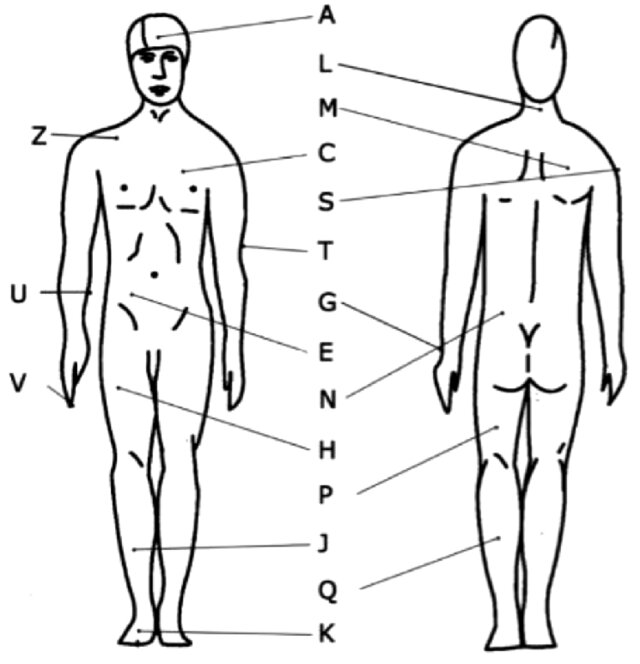
\includegraphics[width=0.5\linewidth]{iso-body-temp-sites.png}
    \caption{Enter Caption}
    \label{fig:enter-label}
\end{figure}

\section{Dashboard}
To facilitate real-time monitoring, a web dashboard will be made where the institutions can track the vitals of all the HCPs working at that time using the data being collected by smart patch in real-time. It will present options to get alerts when an HCP’s vital signs go beyond the threshold. Overall,  the dashboard serves as a central hub for visualizing and interpreting the data collected by the smart patch, facilitating informed decision-making and proactive measures to support the health and well-being of HCPs in high-stress environments. \\ \\
The Agile methodology of the Software Development Lifecycle (SDLC) (refer to \textbf{Appendix B}) will be employed for creating both the Smart Patch and the dashboard.

\section{Features of the System} -- UDPATE THIS - IT IS STILL NOT VERY CLEAR WHAT THE SYSTEM IS DOING

Both the Smart Patch and the Dashboard boast a set of functional and non-functional features meticulously designed to ensure seamless real-time monitoring by healthcare professionals (HCPs). These features are categorized into two types: functional and non-functional. Additionally, they are prioritized using the MoSCoW prioritization framework into Must-Have, Should-Have, Could-Have, and Won’t-Have categories, as illustrated in the \textbf{Appendix \ref{app:features}}. \\ \\
Some of these features have been articulated as user stories, providing a user-centric perspective on the system's capabilities. These user stories, along with their priorities, are presented in Table~\ref{tab:longtable}.

\begin{longtable}{|c|p{9cm}|c|}
\caption{User Stories for VitalMonitor} \label{tab:longtable} \\
\hline
\textbf{User Role} & \textbf{Story} & \textbf{Priority}\\ 
\hline
\endfirsthead

\multicolumn{3}{c}%
{{\bfseries Table \thetable\ Continued from previous page}} \\
\hline
\textbf{User Role} & \textbf{Story} & \textbf{Priority}\\
\hline
\endhead

\hline
\multicolumn{3}{|r|}{{Continued on next page}} \\ \hline
\endfoot

\hline
\endlastfoot

Admin & I want to register my organization.  & Must Have \\ 
\hline
Admin & I want to log in to the dashboard. & Must Have \\
\hline
Admin & I want to add new users. & Must Have \\
\hline
Admin & I want to add new devices. & Must Have \\
\hline
Admin & I want to manage user-device assignments. & Should Have \\
\hline
Admin & I want to monitor vital signs in real-time. & Must Have \\
\hline
Admin & I want to securely log out.  & Should Have \\
\hline
Admin & I want to view a summary of users and devices. & Could Have \\ \hline
User & I want to wear the device comfortably on my ear. & Wont Have \\
\hline
User & I want to easily activate the Smart Patch by pressing a button. & Should Have \\
\hline
User & I want to press the button again to stop sending data. & Should Have \\
\hline
User & I want the device to continuously measure my heart rate and body temperature while activated. & Must Have \\
\hline
\end{longtable}


\section{Evaluation}

To ensure the robustness, reliability, and effectiveness of the Smart Patch and the dashboard, a comprehensive testing and quality assurance process will be implemented throughout the implementation and testing stage of the project:
\begin{itemize}
    \item \textbf{Unit tests:} Conducted to validate the correctness of individual components and the functionality of the Smart Patch and dashboard.
    \item \textbf{Integration testing:} Conducted to verify the seamless integration of components and modules within the Smart Patch and the dashboard.
    \item \textbf{System testing:} Conducted to assess the overall functionality and the performance of the integrated Smart Patch and the dashboard.
    \item \textbf{Acceptance Testing:} Covering all user stories to ensure that the system meets user requirements.
    \item \textbf{Manual testing:} For features that cannot be adequately tested using the above tests.
\end{itemize} 
A systematic evaluation of legal and ethical considerations will also take place:
\begin{enumerate}
    \item \textbf{Legal considerations:} Medical Regulations outlined by MHRA and GDPR guidelines will be followed (see \textbf{Appendix D}).
    \item \textbf{Ethical considerations:} Guidelines provided by the University of Sheffield will be followed, and an ethics application will be made if the project starts to use real human health data other than the developers' data (see \textbf{Appendix E}).
\end{enumerate}


